\section{Torus and it's Automorphisms}
\begin{definition}
Define the torus, $T^2$ as the quotient space $\R^2/\Z^2$ where two points are equivalent if their difference is in $\Z^2$.
\end{definition}
Note that this is homeomorphic to the usual definition $S^1 \times S^1$. The universal covering space of $T^2$ is $\R^2$ and it's fundamental group is $\Z^2$. We identify the equivalance class of the closed curve $\gamma(t)$ based at $[(0,0)]$ with $\tilde{\g}(1)\in \Z^2$, where $\tilde{\g}$ is the lift of $\g$ based at $(0,0)$ in $\R^2$. This map, from $\pi_1(T^2) \to \Z^2$ is a bijection since $\R^2$ is simply connected (see theorem 54.4 on pg 345 in \cite{munkres}).\\

  Automorphisms on the torus correspond to elements in $GL_2(\Z)$. Suppose that $\p:T^2 \to T^2$ is an automorphism then it induces a map $\p_* :\pi_1(T^2) \to \pi_1(T^2)$ which is an isomorphism. Since isomorphisms of $\Z^2$ are just invertible integer matrices. These are just $GL_2(\Z)$ which is the same as matrices with determinant $\pm 1$. On the other hand any $A\in GL_2(\Z)$ will induce an automorphism $\p_A$ on $T^2$ where the mapping is just $[(x,y)] \mapsto [(x,y)A^t]$. The automorphism is orientation preserving if and only if the corresponding matrix $A$ has positive determinant, i.e. $1$.
\begin{proposition}
  The correspondence $\aut(T^2) \to GL_2(\Z)$ is a homomorphism. Moreover if $A$ is in $GL_2(\Z)$ then $(\p_A)_* = A$; i.e. the correspondence is surjective.
\end{proposition}
\begin{proof}
  Since $\l(\phi\circ \psi\r)_*[\g] = [\p\circ\psi \circ \g] = \p_*\circ \psi_*([\g])$ it follows that the map $\p \mapsto \p_*$ is a homomorphism. Let $A$ be $GL_2(\Z)$, then $\p_A$ is well defined automorphism of the torus. Now $\p_{A*}$ acts on $(m,n)\in \Z^2$ in the following way: $(m,n)$ corresponds to the unique class $[\g]$ where $\tilde{\g}(1) = (m,n)$, so the action is given by $\p_{A*}(m,n) = \widetilde{\p_A\circ\gamma}(1)$. Since $\p_A \circ \gamma(t) = \g(t)A^t$, the lifting of this at $(0,0)$ will be just $\tilde{\g}(t) A^t$ (since liftings are unique and this is a lift). Thus $\p_{A*}(m,n) = (m,n)A^t$. Thus $\p_{A*}$ just corresponds to the matrix $A$ in $GL_2(\Z)$.
\end{proof}
Let $A$ be a matrix in $SL_2(\Z)$ and $\p_A$ be the corresponding orientation preserving automorphism, then we can classify $\p_A$ by looking at the properties of the matrix $A$. The characteristic equation of such a matrix is given by $x^2 - \tau x + 1$, where $\tau$ is the trace. We break this into three possibilities:
\begin{enumerate}
  \item $\tau = 0, \pm 1$. In this case the characteristic equation is $x^2 +1$, $x^2-x+1$, or $x^2 + x+ 1$. Thus the eigenvalue are complex in this case. Using Cayley-Hamilton theorem $A$ solves its characteristic equation. In each case we have $A^4 = I$, $A^6=I$, or $A^3=I$ resp.; hence $A^{12} = I$ in each case. Thus the map $\p_A$ is also a finite order map. In this case $\p_A$ is said to be periodic.
  \item $\tau = \pm 2$. In this case the characteristic is $(x\pm 1)^2$. Both eigenvalues are either $1$ or both are $-1$ respectively. Eigenvector of $A$ is integeral and thus correspond to (class of) closed curves on $T^2$. The map preserves the (equivalance class of the) curve (reverses the direction when $\tau = -2$) represented by the eigenvector. No other curve is preserved under the map. These are powers of the Dehn Twists in $C$. 
    \begin{definition}
      A Dehn Twist along a curve $\g$ is defined in the following way: Let $A$ be a regular neighborhood containing $C$ such that $A$ is homeomorphic to an annulus parametrized as $(r,\theta)$. The the extension of the homeomorphism $\p(r,\theta) = (r,\theta + 2\pi r)$ to the whole of the torus (via characteristic function on $A$), is called the Dehn twist.
    \end{definition}
    Matrices corresponding to Dehn twists which preserve the curves corresponding to $(1,0)$ and $(0,1)$ are
    \begin{align*}
      T = \begin{pmatrix}
        1 & 0\\ 1 & 1
      \end{pmatrix}
      \And
      S = \begin{pmatrix}
        1 & -1\\ 0 & 1
      \end{pmatrix}
    \end{align*}
    respectively. \textit{These matrices generate $SL_2(\Z)$ as a group}.
    \begin{figure}
      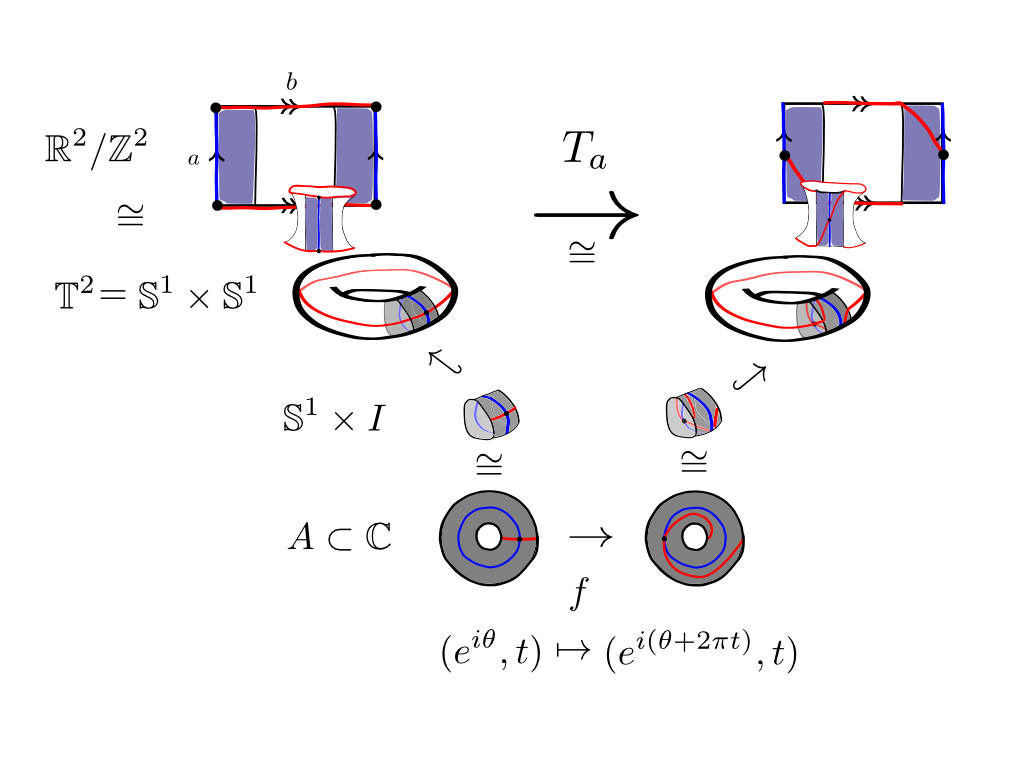
\includegraphics[scale=0.5]{figures/Dehn_twist_for_the_torus.png}
      \caption{Dehn twist along the class of curves represented by $(1,0)$ (blue). The red curve is in the class represented by $(0,1)$. Source of image is wikipedia.}
    \end{figure}
  \item $|\tau| > 2 $. In this case the eigenvalues are distinct reals. The eigenvalues satisfy the relation $\lambda_1\lambda_2 = 1$. Let $|\lambda_1|> 1$. Thus the eigenvalues are of the form $\lambda, 1/\lambda$. Let $v_1,v_2$ be the corresponding eigenvectors. Think of these as elements of $T_{p}(\R^2/\Z^2)$ (tangent space). Consider the curves $\g_i = v_i t $. The action of the map $\p_A$ on $\g_1$ expands it by a factor of $\lambda$ and on $\g_2$ it contracts it by $\lambda^{-1}$. Such maps are called \textit{Anosov Maps}.
\end{enumerate}
